\documentclass[tikz,border=5pt]{standalone}
\usepackage{pgfplots}
\pgfplotsset{compat=1.18}
\usepackage{fontspec}
\setsansfont{SourceSansPro}[
  Path = /usr/local/texlive/2024/texmf-dist/fonts/opentype/adobe/sourcesanspro/,
  UprightFont = SourceSansPro-Regular.otf,
  BoldFont = SourceSansPro-Bold.otf,
  ItalicFont = SourceSansPro-RegularIt.otf,
  BoldItalicFont = SourceSansPro-BoldIt.otf,
  Scale = 1.0
]
\usetikzlibrary{positioning}
\usepackage{xcolor}
\definecolor{primaryblue}{HTML}{012169}
\definecolor{primarygold}{HTML}{B9975B}
\definecolor{highlightyellow}{HTML}{F2A900}
\definecolor{lightbg}{HTML}{E8EDF5}
\definecolor{jet}{HTML}{1A1A1A}
\definecolor{positivegreen}{HTML}{15803D}
\definecolor{negativered}{HTML}{B91C1C}
\begin{document}
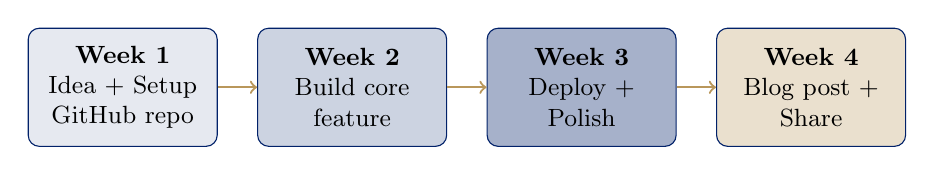
\begin{tikzpicture}[
  box/.style={draw=primaryblue, rounded corners=4pt, fill=lightbg,
              minimum width=2.4cm, minimum height=1.5cm,
              font=\small, align=center},
  arr/.style={->, thick, color=primarygold}
]
  \node[box, fill=primaryblue!10]  (w1) {\textbf{Week 1}\\Idea + Setup\\GitHub repo};
  \node[box, fill=primaryblue!20, right=0.5cm of w1] (w2) {\textbf{Week 2}\\Build core\\feature};
  \node[box, fill=primaryblue!35, right=0.5cm of w2] (w3) {\textbf{Week 3}\\Deploy +\\Polish};
  \node[box, fill=primarygold!30, right=0.5cm of w3] (w4) {\textbf{Week 4}\\Blog post +\\Share};
  \draw[arr] (w1) -- (w2);
  \draw[arr] (w2) -- (w3);
  \draw[arr] (w3) -- (w4);
\end{tikzpicture}
\end{document}
